%%%%%%%%%%%%%%%%%%%%%%%%%%%%%%%%%%%%%%%%%%%%%%%%%%%
%
%  New template code for TAMU Theses and Dissertations starting Spring 2021.  
%
%
%  Author: Thesis Office
%  
%  Last Updated: 1/13/2021
%
%%%%%%%%%%%%%%%%%%%%%%%%%%%%%%%%%%%%%%%%%%%%%%%%%%%
%%%%%%%%%%%%%%%%%%%%%%%%%%%%%%%%%%%%%%%%%%%%%%%%%%%%%%%%%%%%%%%%%%%%%%
%%                           SECTION III
%%%%%%%%%%%%%%%%%%%%%%%%%%%%%%%%%%%%%%%%%%%%%%%%%%%%%%%%%%%%%%%%%%%%%

\chapter{VERY, VERY, VERY LONG TITLE THAT FLOWS INTO A SECOND LINE FOR THE SAKE OF EXAMPLE}

Notice that the title of this section is long - much longer than the others. When you have long section titles, this template takes care of double spacing the lines in the title. If the title is long to fit in the table of contents, the template will single space the title.

\section{Yet Another Table}

Another table is placed here to show the effect of having tables in multiple sections. The list of tables should still double space between table titles, while single spacing long table titles.

%Fix table labeling.
\begin{table}[h!]
	\centering
	\begin{tabular}{|l|l|}
		\hline
		Dates & Attendance  \\ \hline
		August 8-10, 2008 & 3,523  \\ \hline
		August 14-16, 2009 & 4,003 \\ \hline
		July 9-11, 2010 & 5,049 \\ \hline
		August 5-7, 2011 & 6,891  \\ \hline
		August 10-12, 2012 & 9,464  \\ \hline
		August 16-18, 2013 & 11,077  \\ \hline
		July 18-20, 2014 & 14,686 \\ \hline
		July 31-August 2, 2015 & 18,411  \\ \hline
	\end{tabular}
	\caption{San Japan attendance. Data is taken from \cite{neel}. I intentionally make the title of this table long so the single space effect is seen in the list of tables.}
\end{table}

You may be wondering why San Japan was chosen. There are a few reasons as to why I did this:

\begin{enumerate}
\item It is one of the fastest-growing anime conventions in Texas.
\item Filler.
\item I wanted a good variety of table examples.
\item Because conventions are cool.
\end{enumerate}

The \textit{enumerate} environment was used to generated an ordered list above.

\section{Section Test Example}
We insert another figure here, just for kicks.

\begin{figure}[h!]
	\centering
	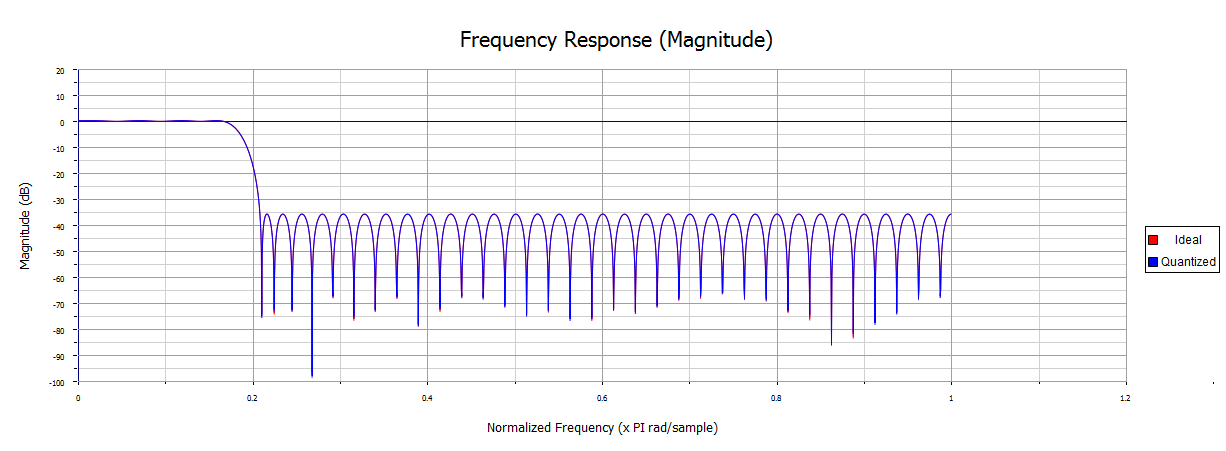
\includegraphics[width = 6.0in]{LowPass_Filter_Design.png}
	\caption{A low pass filter design.}
\end{figure}

\subsection{Filler, Filler, Filler}

This section has filler text. These words serve no meaning except to fill a few lines in the document. This section has filler text. These words serve no meaning except to fill a few lines in the document. This section has filler text. These words serve no meaning except to fill a few lines in the document.

\begin{figure}[h!]
	\centering
	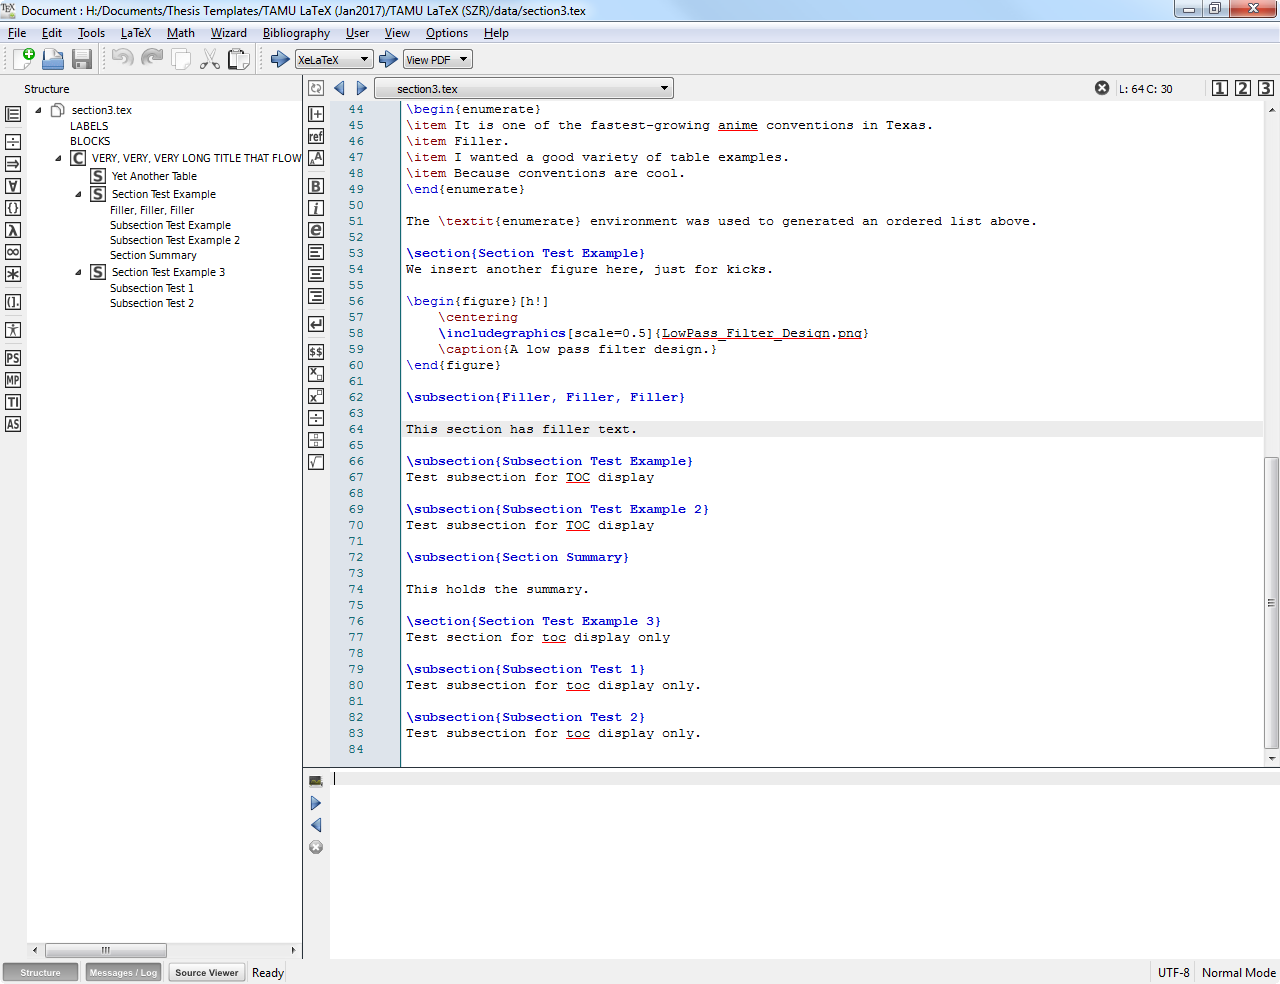
\includegraphics[width=3.75in]{Workspace1.png}
	\caption{A typical Texmaker workspace in Windows 7. The right sidebar displays the current file's structure according to the subsections in place.}
\end{figure}

This section has filler text. These words serve no meaning except to fill a few lines in the document. This section has filler text. These words serve no meaning except to fill a few lines in the document. This section has filler text. These words serve no meaning except to fill a few lines in the document. This section has filler text. These words serve no meaning except to fill a few lines in the document. This section has filler text. These words serve no meaning except to fill a few lines in the document. This section has filler text. These words serve no meaning except to fill a few lines in the document.

\begin{figure}[h!]
	\centering
	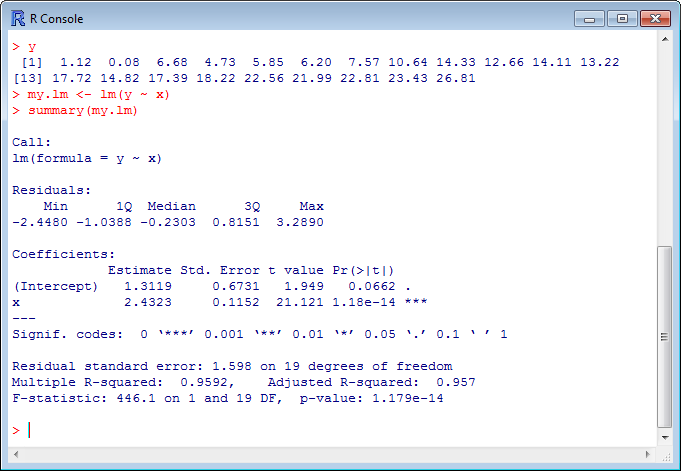
\includegraphics[width=3.5in]{Rachl1.png}
	\caption{Some commands in R.}
\end{figure}

\subsection{Subsection Test Example}
Test subsection for TOC display

\subsection{Subsection Test Example 2}
This section has filler text. These words serve no meaning except to fill a few lines in the document. This section has filler text. These words serve no meaning except to fill a few lines in the document. This section has filler text. These words serve no meaning except to fill a few lines in the document.

\begin{figure}[h!]
	\centering
	
\includegraphics[scale=0.85]{TAM_Logo1.png}
	\caption{The logo of a familiar university.}
\end{figure}

\begin{figure}[!h]
	\caption{Yet another blank float that has no purpose. This is only to test the appearance of the Lists of Figures and the List of Tables.}
\end{figure}

\subsection{Section Summary}
  
This holds the summary. Well, not really a summary - there was a lot of filler in this section.

\begin{figure}[h!]
	\centering
	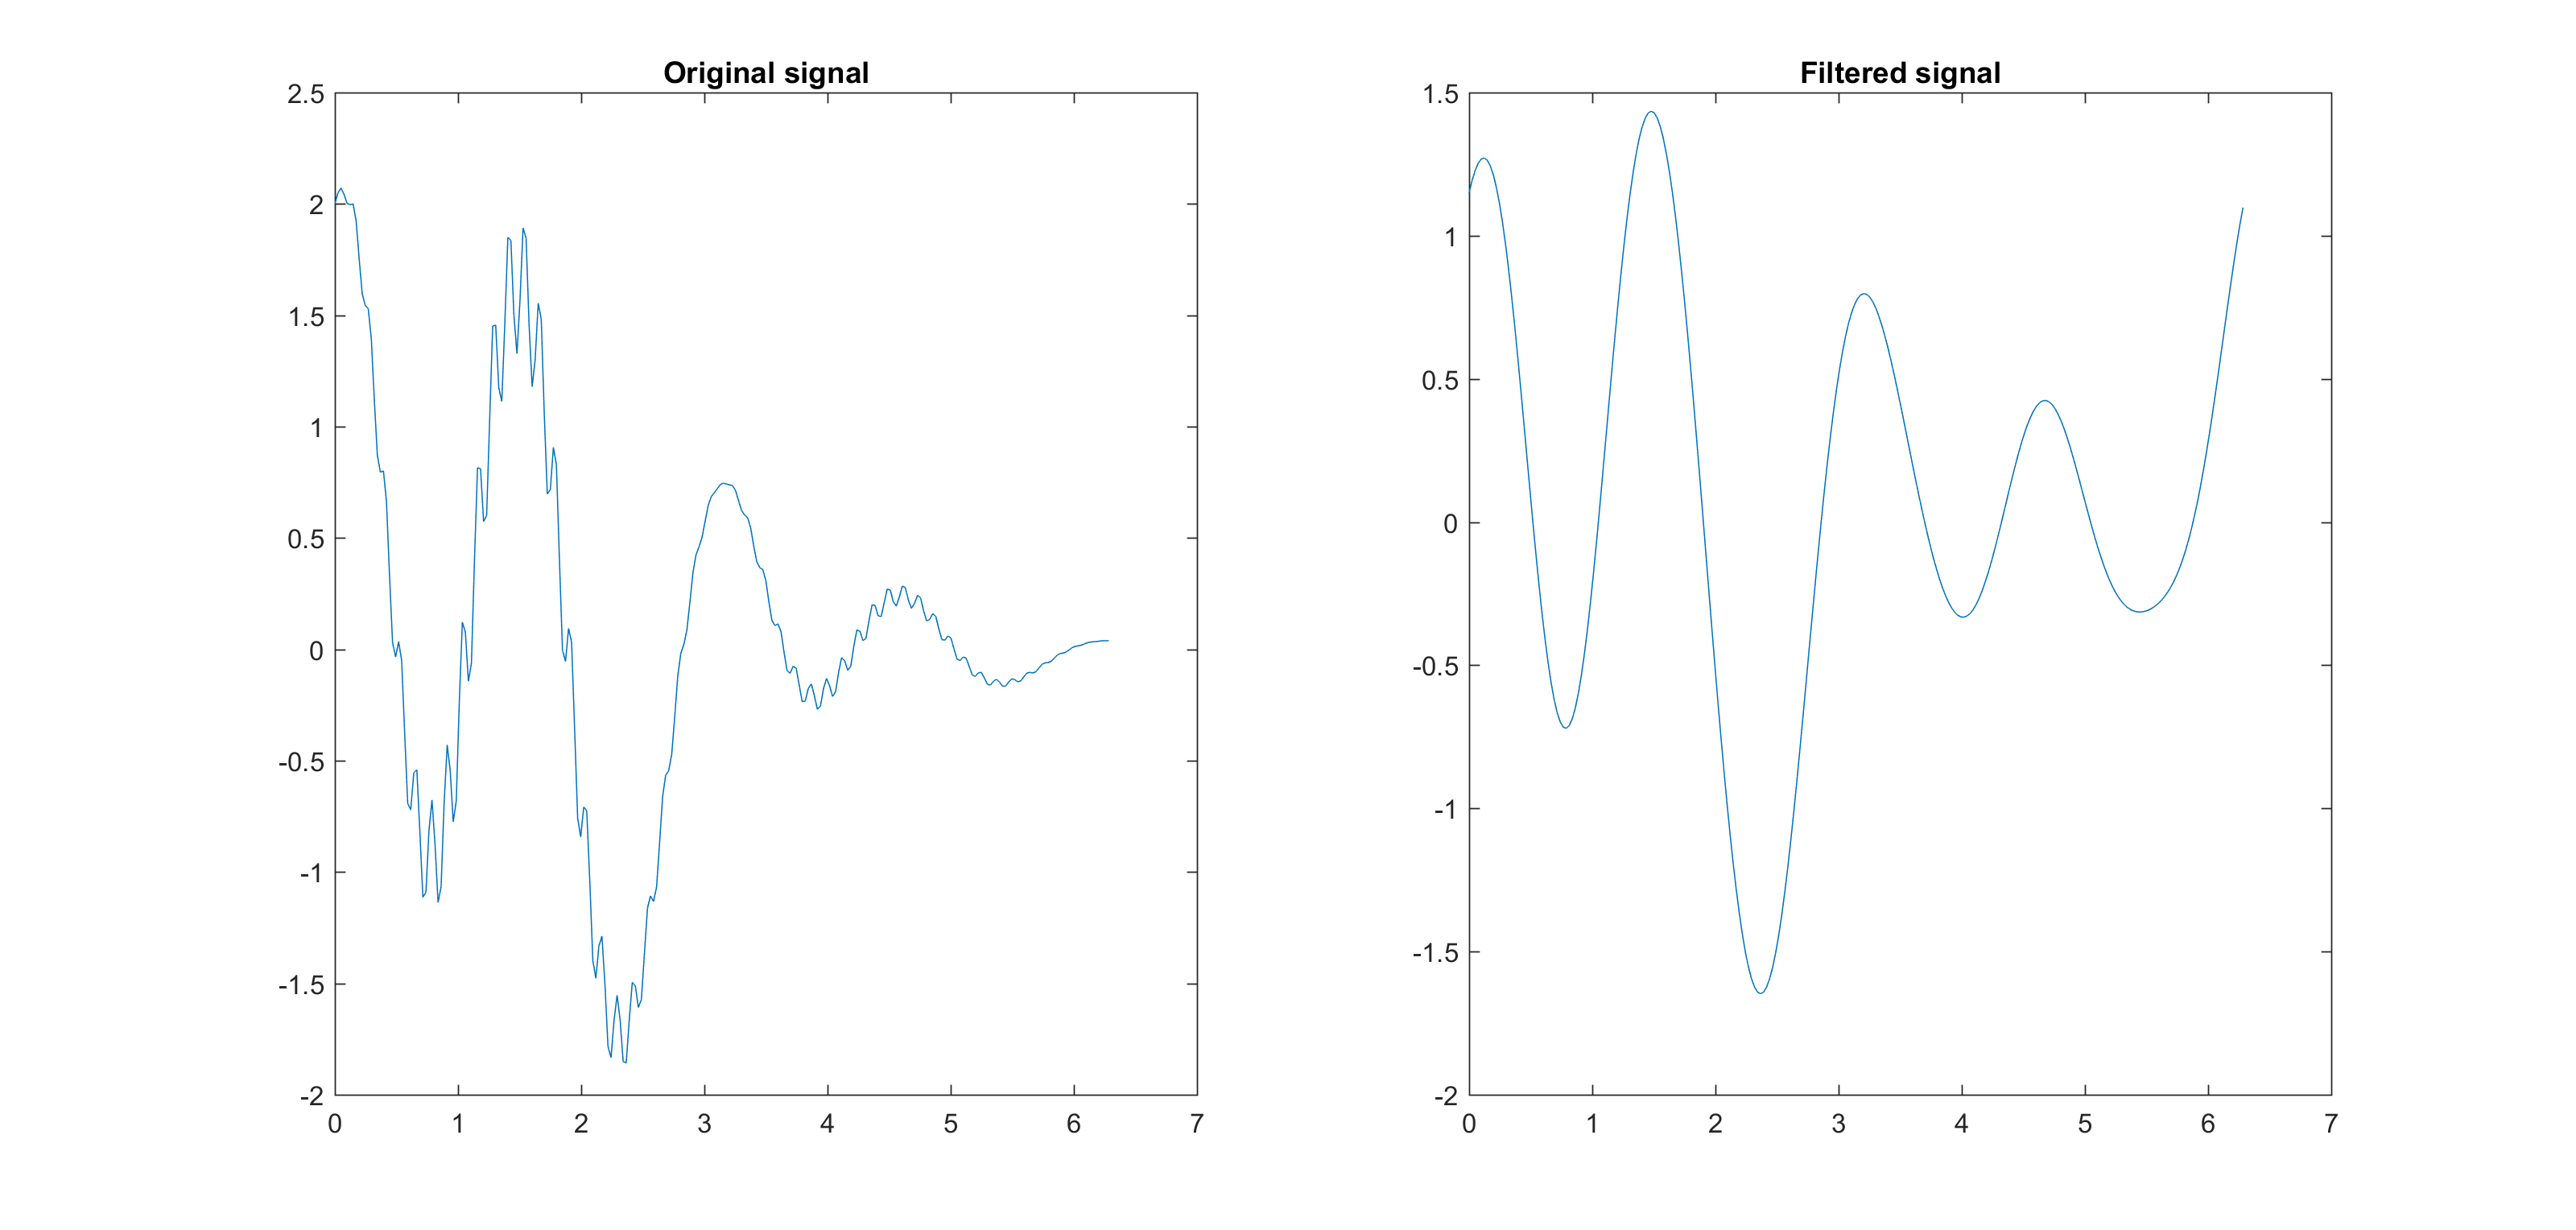
\includegraphics[width=6.5in]{Filter1.png}
	\caption{A signal and the result after a basic filter. The FFT was used to create the plot on the right.}
\end{figure}

\section{Section Test Example 3}
Test section for toc display only.

\begin{figure}[!h]
	\caption{There is nothing to see here.}
\end{figure}

\begin{figure}[!h]
	\caption{There is another float here. I wonder what could be here? Guess what? Nothing! There is no material in this float.}
\end{figure}

\subsection{Subsection Test 1}
Test subsection for toc display only.

\subsection{Subsection Test 2}
Test subsection for toc display only.
